% Generated from figures/generated/batch.svg; do not hand edit.
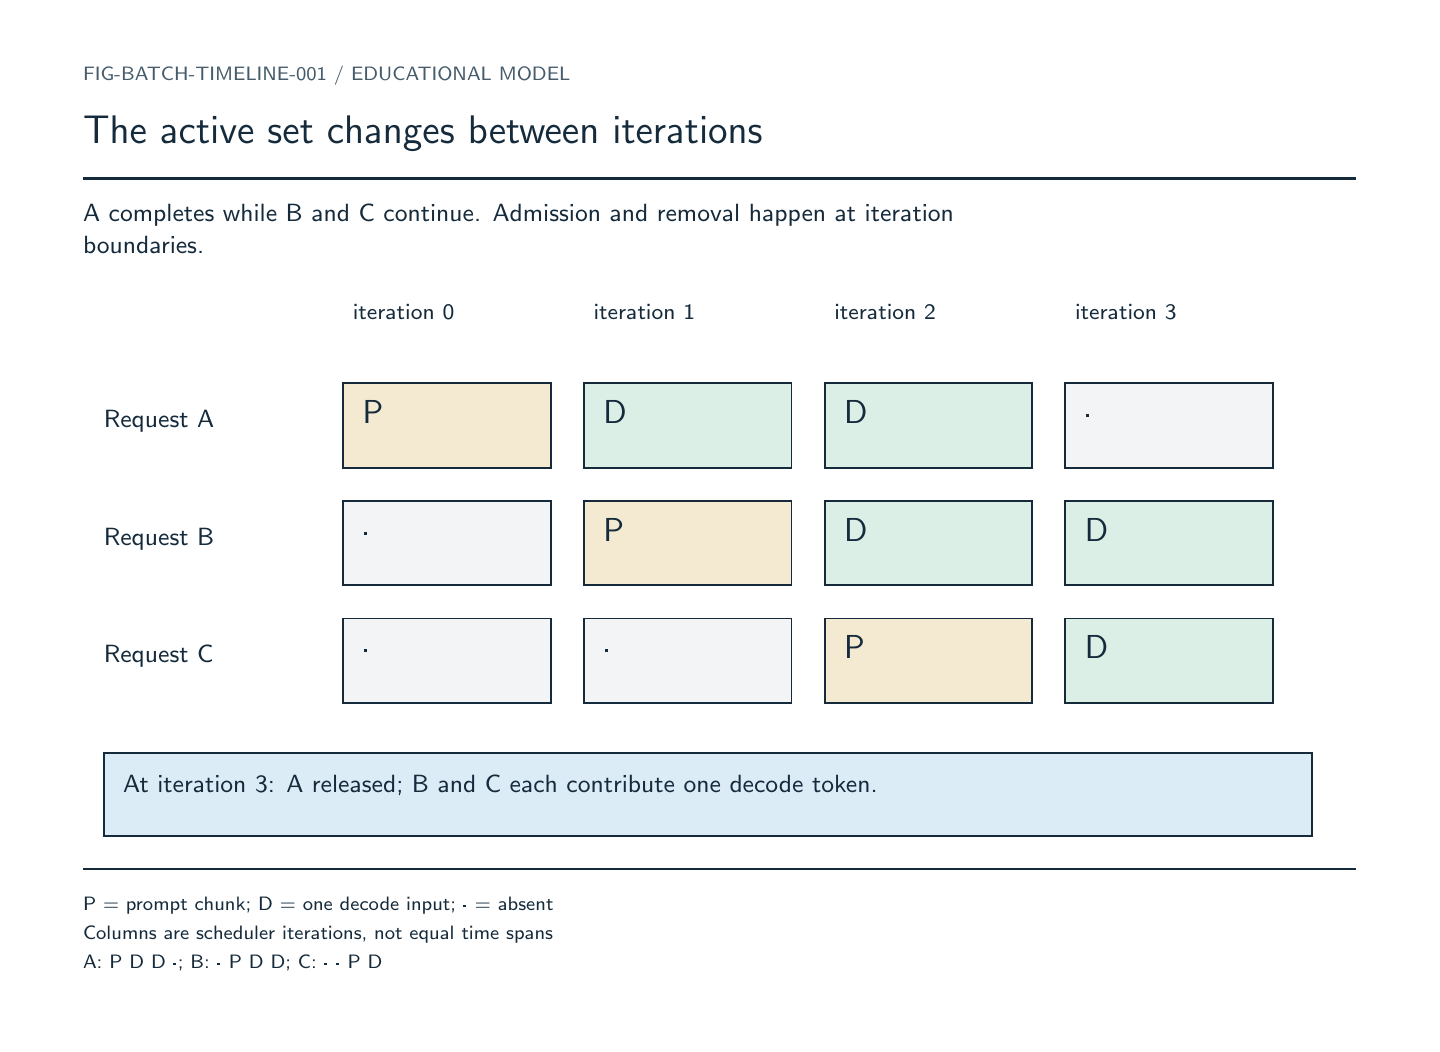
\begin{tikzpicture}[x=.5pt,y=-.5pt]
\path[use as bounding box] (0,0) rectangle (1000,720);
\path[fill=white,draw=none,line width=0.5pt] (0.0,0.0) rectangle (1000.0,720.0);
\node[inner sep=0pt,outer sep=0pt,anchor=base west,text={rgb,255:red,70;green,92;blue,107},font=\sffamily\fontsize{7.0}{8.4}\selectfont] at (40,38) {FIG-BATCH-TIMELINE-001  /  EDUCATIONAL MODEL};
\node[inner sep=0pt,outer sep=0pt,anchor=base west,text={rgb,255:red,21;green,43;blue,60},font=\sffamily\fontsize{15.0}{18.0}\selectfont] at (40,84) {The active set changes between iterations};
\draw[fill=none,draw={rgb,255:red,21;green,43;blue,60},line width=0.75pt] (40,109) -- (960,109);
\node[inner sep=0pt,outer sep=0pt,anchor=base west,text={rgb,255:red,21;green,43;blue,60},font=\sffamily\fontsize{9.5}{11.4}\selectfont] at (40,140) {A completes while B and C continue. Admission and removal happen at iteration};
\node[inner sep=0pt,outer sep=0pt,anchor=base west,text={rgb,255:red,21;green,43;blue,60},font=\sffamily\fontsize{9.5}{11.4}\selectfont] at (40,163) {boundaries.};
\node[inner sep=0pt,outer sep=0pt,anchor=base west,text={rgb,255:red,21;green,43;blue,60},font=\sffamily\fontsize{8.5}{10.2}\selectfont] at (235,211) {iteration 0};
\node[inner sep=0pt,outer sep=0pt,anchor=base west,text={rgb,255:red,21;green,43;blue,60},font=\sffamily\fontsize{8.5}{10.2}\selectfont] at (409,211) {iteration 1};
\node[inner sep=0pt,outer sep=0pt,anchor=base west,text={rgb,255:red,21;green,43;blue,60},font=\sffamily\fontsize{8.5}{10.2}\selectfont] at (583,211) {iteration 2};
\node[inner sep=0pt,outer sep=0pt,anchor=base west,text={rgb,255:red,21;green,43;blue,60},font=\sffamily\fontsize{8.5}{10.2}\selectfont] at (757,211) {iteration 3};
\node[inner sep=0pt,outer sep=0pt,anchor=base west,text={rgb,255:red,21;green,43;blue,60},font=\sffamily\fontsize{9.5}{11.4}\selectfont] at (55,289) {Request A};
\path[fill={rgb,255:red,244;green,234;blue,210},draw={rgb,255:red,21;green,43;blue,60},line width=0.7pt] (228.0,257.0) rectangle (378.0,318.0);
\node[inner sep=0pt,outer sep=0pt,anchor=base west,text={rgb,255:red,21;green,43;blue,60},font=\sffamily\fontsize{12.0}{14.399999999999999}\selectfont] at (242,286) {P};
\path[fill={rgb,255:red,220;green,239;blue,231},draw={rgb,255:red,21;green,43;blue,60},line width=0.7pt] (402.0,257.0) rectangle (552.0,318.0);
\node[inner sep=0pt,outer sep=0pt,anchor=base west,text={rgb,255:red,21;green,43;blue,60},font=\sffamily\fontsize{12.0}{14.399999999999999}\selectfont] at (416,286) {D};
\path[fill={rgb,255:red,220;green,239;blue,231},draw={rgb,255:red,21;green,43;blue,60},line width=0.7pt] (576.0,257.0) rectangle (726.0,318.0);
\node[inner sep=0pt,outer sep=0pt,anchor=base west,text={rgb,255:red,21;green,43;blue,60},font=\sffamily\fontsize{12.0}{14.399999999999999}\selectfont] at (590,286) {D};
\path[fill={rgb,255:red,242;green,244;blue,245},draw={rgb,255:red,21;green,43;blue,60},line width=0.7pt] (750.0,257.0) rectangle (900.0,318.0);
\node[inner sep=0pt,outer sep=0pt,anchor=base west,text={rgb,255:red,21;green,43;blue,60},font=\sffamily\fontsize{12.0}{14.399999999999999}\selectfont] at (764,286) {·};
\node[inner sep=0pt,outer sep=0pt,anchor=base west,text={rgb,255:red,21;green,43;blue,60},font=\sffamily\fontsize{9.5}{11.4}\selectfont] at (55,374) {Request B};
\path[fill={rgb,255:red,242;green,244;blue,245},draw={rgb,255:red,21;green,43;blue,60},line width=0.7pt] (228.0,342.0) rectangle (378.0,403.0);
\node[inner sep=0pt,outer sep=0pt,anchor=base west,text={rgb,255:red,21;green,43;blue,60},font=\sffamily\fontsize{12.0}{14.399999999999999}\selectfont] at (242,371) {·};
\path[fill={rgb,255:red,244;green,234;blue,210},draw={rgb,255:red,21;green,43;blue,60},line width=0.7pt] (402.0,342.0) rectangle (552.0,403.0);
\node[inner sep=0pt,outer sep=0pt,anchor=base west,text={rgb,255:red,21;green,43;blue,60},font=\sffamily\fontsize{12.0}{14.399999999999999}\selectfont] at (416,371) {P};
\path[fill={rgb,255:red,220;green,239;blue,231},draw={rgb,255:red,21;green,43;blue,60},line width=0.7pt] (576.0,342.0) rectangle (726.0,403.0);
\node[inner sep=0pt,outer sep=0pt,anchor=base west,text={rgb,255:red,21;green,43;blue,60},font=\sffamily\fontsize{12.0}{14.399999999999999}\selectfont] at (590,371) {D};
\path[fill={rgb,255:red,220;green,239;blue,231},draw={rgb,255:red,21;green,43;blue,60},line width=0.7pt] (750.0,342.0) rectangle (900.0,403.0);
\node[inner sep=0pt,outer sep=0pt,anchor=base west,text={rgb,255:red,21;green,43;blue,60},font=\sffamily\fontsize{12.0}{14.399999999999999}\selectfont] at (764,371) {D};
\node[inner sep=0pt,outer sep=0pt,anchor=base west,text={rgb,255:red,21;green,43;blue,60},font=\sffamily\fontsize{9.5}{11.4}\selectfont] at (55,459) {Request C};
\path[fill={rgb,255:red,242;green,244;blue,245},draw={rgb,255:red,21;green,43;blue,60},line width=0.7pt] (228.0,427.0) rectangle (378.0,488.0);
\node[inner sep=0pt,outer sep=0pt,anchor=base west,text={rgb,255:red,21;green,43;blue,60},font=\sffamily\fontsize{12.0}{14.399999999999999}\selectfont] at (242,456) {·};
\path[fill={rgb,255:red,242;green,244;blue,245},draw={rgb,255:red,21;green,43;blue,60},line width=0.7pt] (402.0,427.0) rectangle (552.0,488.0);
\node[inner sep=0pt,outer sep=0pt,anchor=base west,text={rgb,255:red,21;green,43;blue,60},font=\sffamily\fontsize{12.0}{14.399999999999999}\selectfont] at (416,456) {·};
\path[fill={rgb,255:red,244;green,234;blue,210},draw={rgb,255:red,21;green,43;blue,60},line width=0.7pt] (576.0,427.0) rectangle (726.0,488.0);
\node[inner sep=0pt,outer sep=0pt,anchor=base west,text={rgb,255:red,21;green,43;blue,60},font=\sffamily\fontsize{12.0}{14.399999999999999}\selectfont] at (590,456) {P};
\path[fill={rgb,255:red,220;green,239;blue,231},draw={rgb,255:red,21;green,43;blue,60},line width=0.7pt] (750.0,427.0) rectangle (900.0,488.0);
\node[inner sep=0pt,outer sep=0pt,anchor=base west,text={rgb,255:red,21;green,43;blue,60},font=\sffamily\fontsize{12.0}{14.399999999999999}\selectfont] at (764,456) {D};
\path[fill={rgb,255:red,220;green,236;blue,247},draw={rgb,255:red,21;green,43;blue,60},line width=0.7pt] (55.0,524.0) rectangle (928.0,584.0);
\node[inner sep=0pt,outer sep=0pt,anchor=base west,text={rgb,255:red,21;green,43;blue,60},font=\sffamily\fontsize{9.0}{10.799999999999999}\selectfont] at (69,553) {At iteration 3: A released; B and C each contribute one decode token.};
\draw[fill=none,draw={rgb,255:red,21;green,43;blue,60},line width=0.75pt] (40,608) -- (960,608);
\node[inner sep=0pt,outer sep=0pt,anchor=base west,text={rgb,255:red,21;green,43;blue,60},font=\sffamily\fontsize{7.5}{9.0}\selectfont] at (40,638) {P = prompt chunk; D = one decode input; · = absent};
\node[inner sep=0pt,outer sep=0pt,anchor=base west,text={rgb,255:red,21;green,43;blue,60},font=\sffamily\fontsize{7.5}{9.0}\selectfont] at (40,659) {Columns are scheduler iterations, not equal time spans};
\node[inner sep=0pt,outer sep=0pt,anchor=base west,text={rgb,255:red,21;green,43;blue,60},font=\sffamily\fontsize{7.5}{9.0}\selectfont] at (40,680) {A: P D D ·; B: · P D D; C: · · P D};
\end{tikzpicture}
